\documentclass[12pt,a4paper]{article}

\usepackage[utf8]{inputenc}
\usepackage[spanish, es-tabla]{babel}
\usepackage[version=3]{mhchem}
\usepackage[journal=jacs]{chemstyle}
\usepackage{amsmath}
\usepackage{algpseudocode}
\usepackage{dsfont}
\usepackage{listings}
\usepackage{pdfpages}
\usepackage{amsfonts}
\usepackage{amssymb}
\usepackage{makeidx}
\usepackage{enumitem}
\usepackage{xcolor}
\usepackage[stable]{footmisc}
\usepackage[section]{placeins}

%Paquetes necesarios para tablas
\usepackage{longtable}
\usepackage{array}
\usepackage{xtab}
\usepackage{multirow}
\usepackage{colortab}
\usepackage{caratula}

\usepackage{caratula}
\usepackage[colorlinks=true, linkcolor=blue]{hyperref}
\usepackage{calc}
% * <lucasrafael.romero@gmail.com> 2016-09-01T20:01:11.750Z:
%
% ^.

%Paquetes necesarios para imágenes, pies de página, etc.
\usepackage{graphicx}
\usepackage{lmodern}
\usepackage{fancyhdr}
\usepackage[left=4cm,right=2cm,top=3cm,bottom=3cm]{geometry}

%Instrucción para evitar la indentación
%\setlength\parindent{0pt}
%Paquete para incluir la bibliografía
\usepackage[backend=bibtex,style=chem-acs,biblabel=dot]{biblatex}
\addbibresource{references.bib}

%Formato del título de las secciones

\usepackage{titlesec}
\usepackage{enumitem}
\titleformat*{\section}{\bfseries\large}
\titleformat*{\subsection}{\bfseries\normalsize}

%Creación del ambiente anexos
\usepackage{float}
\floatstyle{plaintop}
\newfloat{anexo}{thp}{anx}
\floatname{anexo}{Anexo}
\restylefloat{anexo}
\restylefloat{figure}

%Modificación del formato de los captions
\usepackage[margin=10pt,labelfont=bf]{caption}

%Paquete para incluir comentarios
\usepackage{todonotes}

\parskip=5pt % 10pt es el tamaño de fuente

% Pongo en 0 la distancia extra entre ítemes.
\let\olditemize\itemize
\def\itemize{\olditemize\itemsep=0pt}

% Acomodo fancyhdr.
\pagestyle{fancy}
\thispagestyle{fancy}
\addtolength{\headheight}{3pt}
\lhead{Laboratorio de Métodos Numéricos}
\rhead{TP 1: Trabajamos y nos divertimos...}
\cfoot{\thepage /\pageref{LastPage}}
\renewcommand{\footrulewidth}{0.4pt}

\author{Grupo 14}
\date{}
\title{TP 1: Trabajamos y nos divertimos...}

\def\Materia{Laboratorio de Métodos Numéricos}
\def\Titulo{Trabajo Práctico Número 1}
\def\Subtitulo{Trabajamos y nos divertimos...}
%\def\Grupo{Grupo 14}
\integrante{Zar Abad, Ciro Román}{129/15}{ciromanzar@gmail.com}
\integrante{Lopez Valiente, Patricio}{457/15}{patricio454@gmail.com}
\integrante{Romero, Lucas Rafael}{440/12}{lucasrafael.romero@hotmail.com}

%%%%%%%%%%%%%%%%%%%%%%
%Inicio del documento%
%%%%%%%%%%%%%%%%%%%%%%

\begin{document}

\lstset{language=C++, breaklines}

\maketitle
%\newpage\null\thispagestyle{empty}\newpage

\tableofcontents

\pagebreak

\section*{\centering Resumen}

En este trabajo presentamos el problema de representar computacionalmente el comportamiento de temperatura dentro de las paredes de un alto horno. El objetivo es encontrar los puntos internos de la pared donde la temperatura alcanza los 500ºC, a lo que llamamos isoterma 500, en base a las mediciones de temperaturas en el exterior de dicha pared. Luego, esta información se utilizará para analizar el riesgo de derrumbe de la estructura.\\
Para ello desarrollamos un modelo para discretizar los puntos de la pared, crear el sistema lineal que representa el problema y analizamos distintos métodos numéricos para resolverlo.

A continuación realizamos experimentaciones para comparar la performance de dichos métodos. Corremos las implementaciones para matrices de distintos tamaños y para instancias similares variando tan solo el vector de resultados. Además comparamos los resultados obtenidos contra los proporcionados por matlab, que es la herramienta de la que disponemos cuyos resultados consideramos son los más acercados a la realidad.\\ 
Finalmente, exponemos nuestras conclusiones.

\section{Introducción teórica}

\subsection{Introducción del problema}

A partir de los datos de un alto horno, lo modelamos como una matriz de puntos discretos tomando una cantidad finita de radios y de ángulos y pretendemos encontrar la isoterma 500. Es decir, los puntos sobre la pared del horno que tienen temperatura de 500 ºC.

Para encontrar estos puntos contamos con la ecuación de Laplace:
\begin{equation}
	\frac{{\partial}^2T(r,\theta)}{\partial r^2} + \frac{1}{r} \frac{\partial T(r,\theta)}{\partial r} + \frac{1}{r^2} \frac{{\partial}^2T(r,\theta)}{{\partial}^2 \theta} = 0
\end{equation}


Esto presenta 2 problemas: No es simple encontrar las derivadas de la función y el dominio de esta son los reales. Teniendo eso en cuenta, nos inclinamos a resolver una aproximación más simple:

\begin{equation}
	\frac{t_{j-1,k} -2t_{j,k} + t_{j+1,k}}{(\Delta r)^2} + \frac{1}{r} \frac{t_{j,k}-t_{j-1,k}}{\Delta r} + \frac{1}{r^2} \frac{t_{j,k-1} -2t_{j,k} + t_{j,k+1}}{(\Delta \theta)^2} = 0
\end{equation}

Esta ecuación nos deja con un sistema lineal que podemos resolver para encontrar la temperatura en cada punto del modelo. A partir de eso, interpolamos los valores para obtener la isoterma buscada.

\subsection{Eliminación Gaussiana}
Uno de los algoritmos posibles para resolver el sistema lineal es la eliminación Gaussiana. Aprovechando el hecho que cambiar las filas de una matriz por combinaciones lineales de estas devuelve un sistema equivalente, es posible operar entre las filas para conseguir una matriz triangular superior equivalente. En definitiva un sistema más simple de resolver.

El algoritmo es el siguiente:
\begin{algorithmic}

\Procedure{Eliminación Gaussiana}{$A \in {\mathds{R}}^{nxn} $}
  \For{$i\;=\;1$ to $n-1$}
  	\For{$i\;=\;1$ to $n-1$}
    
    \State $m_{j,i} \gets \frac{a_{j,i}}{a_{i,i}}$
    \Comment $F_k = e_k A$
    \State $F_j \gets F_j - m_{j,i} \; F_i$
    
    \EndFor
  \EndFor
\EndProcedure
\end{algorithmic}

El algoritmo asume que el elemento k-ésimo de la diagonal luego de la iteración k es distinto de 0. Más adelante demostraremos que es una suposición válida para esta clase de sistemas.

\subsection{Factorización LU}

La factorización LU es similar a la eliminación Gaussina en el sentido que calcula la misma matriz triangular superior de la misma manera. Sin embargo, la factorización LU se guarda los multiplicadores en una matriz triangular inferior L de manera que $A\! =\! L\; U$

De esta manera, tenemos una forma simple de expresar la matriz A. Para resolver el sistema $Ax \! = \! b $ resolvemos:
\begin{align*}
\begin{cases}
Ly = b \\
Ux = y 
\end{cases}
\end{align*}

La ventaja que presenta este enfoque frente a la eliminación gaussiana es que, manteniendo la matriz A, es posible resolver el sistema para distintos vectores b sin tener que recalcular la triangulación.

\section{Desarrollo}

\subsection{Métodos utilizados}

Los métodos numéricos implementados en este trabajo préctico fueron Eliminacion Gaussiana y factorizacion LU. Estos fueron empleados para la busqueda de la isoterma de un Alto Horno y resultaron de gran utilidad, ya que se contó con un método para discretizar la temperatura de las paredes del Alto Horno, de forma que se convertia en un sistema lineal. Esto se logro mediante ecuaciones de calor provistas por la cátedra, y propiedades que cumplen los Altos Hornos. La discretizacion del sistema fue llevada a cabo tomando una serie de radios y ángulos, donde cada punto marcaba una incógnita.

\subsection{Implementación}

Para la implentación de los métodos usados, se empezó primero por definir la clase matriz por sobre los cuales iban a operar, la implementación de la misma no fue una tarea dificil. Como siguiente paso se paso a implementar la Eliminacion Gaussiana y por posterior Factorizacion LU, ya que su implentación una ves que se cuenta con el algoritmo de Eliminacion Gaussiana pasa a ser casi trivial. Posteriormente a esto se paso a implentar los algoritmos para resolver sistemas triangularizados, comunmente conocidos como $"$backward substitution$"$ y $"$forkward substitution$"$.
Como paso final se implementaron las funciones para la carga, creación y escritura del sistema Matricial.

Durante la primera parte de la implentación, los problemas que surgian, no eran de mayor importancia, ya que eran problemas de tipo o similar, por lo que no eran dificiles de localizar, aunque no eran triviales. Lo mismo ocurrio con la implentación  de Eliminacion Gaussiana, Factorizacion LU, $"$backward substitution$"$ y $"$forward substitution$"$. \\
Sin embargo a la hora de implentar los metodos creacion y escritura surgieron problemas que demoraron mucho mas en ser resueltos, esto se debía a que eran de difícil resolución por su poca notoriedad, ya que se debian a una mala interpretacion del sistema en un caso (confundimos radios con angulos), o problemas de precisión en las funciones nativas de C++. Estas resultaron particularmente difíciles de resolver, ya que requirieron que veamos documentacion de C++, y diversos foros como $"$StackOverflow$"$ y similares hasta dar con la solución, ejemplos de este tipo de problemas se dieron con el operador $<<$ y con el operador de Division $/$, que truncaban los resultados al imprimirlos. \\

\subsection{Búsqueda de la isoterma}

A la hora de aproximar la ubicación de la isoterma 500, se analizaron distintos tipos de interpolaciones. Finalmente se optó por utilizar interpolación lineal por su simpleza, y porque en caso de no ser lo suficientemente precisa, esto se puede compensar con una discretización de radios mas fina. \\

La ecuación de interpolación lineal, dado un ángulo $\theta$ fijo, la función $T(r)$ que determina la temperatura de la pared en el punto $(r,\theta)$ y dos radios contiguos $r_1$ y $r_2$ tal que $T(r_2)$ $\geq$ ISO y $T(r_1)$ $<$ ISO (siendo ISO la temperatura de la isoterma buscada, ej: 500) es la siguiente:

\begin{equation}
ISO = {T(r_1)} + \frac{T(r_2) - T(r_1)}{r_2 - r_1}(r - r_1)
\end{equation}

Despejando $r$, y escribiendo ($r_2 - r_1$) como $\Delta r$ queda:

\begin{equation}
r = \frac{(ISO - T(r_1)) \Delta r}{T(r_2) - T(r_1)} + r_1
\end{equation}


\subsection{Evaluación de peligrosidad}

A la hora de proponer un forma de evaluar la peligrosidad de la estructura en funcion de la distancia de la isoterma a la pared externa del horno nos encontramos con problemas y planteos diversos, y aunque se investigo sobre el concepto detras del Alto Horno al desconocer cuestiones ligadas a la fisica y ingenieria de la estructura no podiamos encontrar una forma librada de ambiguedad. Algunas de las primeras ideas que surgieron a un principio fueron: 
   \begin{itemize}
		\item $"$Medir la distancia de la media de la isorterma con respecto a la pared exterior, y si es cercana, decir que peligra la extructura$"$. Ésta fue rapidamente descartada ya que al no conocer que como funciona la disipacion de calor en los Altos Hornos, no podiamos establecer cuando habia o no cercania.
        \item $"$Tomar como medida la cercania de la isoterma mas grande al radio exterior$"$. Tambien fue descartada por razones similares a la anterior, además del hecho de que no es muy expresiva en función de que arrojaría el mismo indice de peligro para una medida en que la isoterma es homogeneamente $"$grande$"$, que para una que presenta un $"$outlier$"$.
        \item $"$Emitir el indice de peligro en funcion de si los valores obtenidos se correspondía con respecto a los de una distribución normal dada por la media y la varianza de la isoterma$"$. Ésta fue descartada no trivialmente, ya que aunque en un principio parecía ser una buena opción permitia que isotermas con formas similires a las de una flor (gran varianza y una media promedio) aparenten ningun peligro cuando en realidad lo hacen.
	\end{itemize}
Finalmente se penso una forma que tenia que ser fiable, y que los conocimientos necesarios para entender su funcionamiento no tenian que depender del conocimiento de la estructura, sino de datos provistos por ella.

Por lo que se ideo el siguiente protocolo para medir el peligro de la estructura:
	\begin{itemize}
		\item 1. Se obtiene apartir de la consulta con un profesional, o del fabricante, datos de la ubicacion de la isoterma en un caso controlado borde, donde el peligro es nulo, pero esta proximo a no serlo. Si no dispusiéramos de estos medios para conseguir el mismo, como conocemos que la temperatura de la pared exterior se encuentra entre 50 ºC y 200 ºC, podriamos suponer que un buen candidato para ser nuestro caso es por ejemplo uno donde las temperaturas de la pared exterior varian entre 160 ºC y 190 ºC, ya que este es un caso que esta cercano a dejar de ser promedio, pero la pared exterior presenta temperaturas mayores a las esperadas . A la media de esta Isoterma la llamaremos ISOCTRL
        \item 2. Apartir de la isoterma ISOCTR mediremos generaremos tres valores:
		\begin{itemize}
			\item ISOMD: que consiste en la resta entre la media de la isoterma medida e ISOCTR. En el caso de ser Negativo, se le asigna 0.
            \item ISOMAX: que consiste en la resta entre el maximo de la isoterma medida e ISOCTR. En el caso de ser Negativo, se le asigna 0.
            \item NRMISO: que consiste en la resta entre el radio exterior e ISOCTR.(esta se usara para normalizar el Indice)
    	\end{itemize}
        \item 3. Ahora de esta forma se obtiene el siguiente indice de peligro:
        
        $IPREGULAR = \frac{ISOMD}{NRMISO}$
        
        
        $IPLOCAL = \frac{ISOMAX}{NRMISO}$
        
        donde IPREGULAR e IPLOCAL varían entre 0 y 1, y a medida que estos crecen, el peligro de rotura en la estructura lo hace tambien.
        De esta forma al disponer de estos dos indices, se puede obtener informacion adicional, por ejemplo si los dos indices son similares se podria inferir que la perdida de calor es homogeneamente alta o normal dependiendo de que valor entre 0 y 1 nos den. De la misma forma en un caso donde IPREGULAR es relativamente mas chico que IPLOCAL, se podria inferir que posiblemente hay un segmento de la pared que no esta disipando el calor de forma adecuada. 
	\end{itemize}
    
\subsection{Experimentos}    
%
Los experimentos llevados a cabo fueron ideados siguiendo los siguientes lineamientos:
\begin{itemize}
	\item Para los experimentos referidos a la busqueda de la isoterma 500 y los posibles efectos que podia tener la granulacion del sistema sobre la presicion de la misma se decidieron llevar a cabo cuatro macro experimentos, los cuales consistian en distintas formas de discretizar sistemas en funcion de los radios y angulos, cada uno de ellos divididos en dos casos:
\begin{itemize}
\item Caso A: Presentando un sistema equilibrado con temperaturas dentro del rango de lo esperado.
\item Caso B: Una medición en la pared externa con picos en las temperaturas y que presentan una posible situación de riesgo (igual para todos los experimentos, pero con mayor o menor cantidad de sensores dependiendo del caso).
	\end{itemize}

	Para cada uno de estos casos, las discretizaciones elegidas fueron las siguientes: 
    \begin{itemize}
		\item Exp. 1: donde la cantidad ángulos y radios tomados era pequeña (10 ángulos y 10 radios).
        \item Exp. 2: donde la cantidad ángulos y radios tomados era grande (50 ángulos y 50 radios).
        \item Exp. 3: donde la cantidad ángulos era grande y de radios pequeña (100 ángulos y 20 radios).
        \item Exp. 4: donde la cantidad ángulos era pequeña y de radios grande (20 ángulos y 100 radios).
	\end{itemize}

    Para su realización se construyeron los sistemas y se los resolvio utilizando el método de Eliminación Gaussiana. Luego se realizaron las correspondientes imágenes que grafican los resultados obtenidos.  \\
    
    Dado que los resultados obtenidos difirieron bastante de lo que habíamos esperado encontrarnos en base a nuestra intuición, optamos por realizar un experimento nuevo para reforzar las concluciones. \\
    
    Basandonos en el caso B de los experimentos anteriores, dividimos el nuevo experimento en dos etapas:
    \begin{itemize}
    	\item Exp. 5: dejando fijo la cantidad de ángulos y variando la de radios.
	    \item Exp. 6: dejando fijo la cantidad de radios y variando los ángulos.
   	\end{itemize}
En estos nuevos casos, optamos por superponer los gráficos para poder compararlos mas eficientemente.
    
   \item Para los experimentos concernientes a la efectividad en terminos de complejidad temporal de la Eliminacion Gaussiana y la Factorizacion LU, se llevaron a cabo tres experimentos en los que se buscaba ver la efectividad de estos para diferentes aspectos:
    \begin{itemize}
		\item El experimento numero uno se ideo con el fin de ver como crecia la complejidad de temporal de la Eliminacion Gaussiana y la Factorizacion LU, en funcion del tamaño del sistema a resolver, es decir de la Matriz que definia el sistema, para ello se midio el tiempo que los metodos implementados tardaban en resolver una sola instancia para matrices de tamaños que variaban desde 9x9 hasta 1600x1600.
		\item El experimento numero dos se ideo para ver como respondian nuestro metodos numericos ante una medicion de un sistema para un gran numero de instancias, para ellos se midio el tiempo que tardaban en resolver j instancias distintas, para una matriz de 30x30, con $1$ $\leq$ j $\leq$ $25$.   
        \item El experimento numero tres se presento como un experimento posible apartir de observar los primeros resultados del experimento dos, al observar las difencias entre los metodos propuestos para cuando se instanciaba a la misma matriz del sistema con mas de una instacia. Para ello se midio el tiempo que tardaba en dar con el resultado particular de cada instancia, una matriz de 30x30 y 10 instancias.
        \item El experimento número 4 pretende comparar los resultados obtenidos por las implementaciones de fact. LU y eliminación gaussiana contra los resultados arrojados por Matlab para los mismos sistemas. Para eso, se calcularon 2 instancias distintas mediante los distintos métodos (cabe destacar que los resultados de nuestras implementaciones fueron idénticos) y tomamos la diferencia relativa\footnote{restar los resultados de los vectores y dividir el vector por uno de los vectores resultados} entre ellos.
	\end{itemize}
para la medicion de tiempos se empleo la librerias $"chrono"$ y $"ctime"$ de $c++$, estas mismas cuentan con diversas funciones para la medicion de tiempos dentro del codigo, fueron empleados estos procesos y no otros conocidos como el comando $"time"$ de bash u otros, ya que al permitir mediciones en el codigo no solo ofrecian a priori un resultado mas fiable y menos permeable a procesos externos, sino que dada su maleabilidad facilitaban enormemente la toma de mediciones.

    \item Finalmente, con el objetivo de analizar la exactitud de nuestros algoritmos para resolver sistemas lineales, realizamos dos experimentos que consistieron en generar un sistema pequeño, resolverlo usando los dos métodos implementados (EG y LU) y compararlos con los resultados obtenidos resolviendo el mismo sistema con Matlab.

\end{itemize}
%%%%%%%%%%%%%%%%%%%%%%%%%%%%%%%%%%%%%%
%Deben explicarse los metodos numericos que utilizaron y su aplicacion al problema concreto involucrado en el trabajo practico. Se deben mencionar los pasos que siguieron para implementar los algoritmos, las dificultades que fueron encontrando y la descripcion de como las fueron resolviendo. Explicar tambien como fueron planteadas y realizadas las mediciones experimentales. 
%Los ensayos fallidos, hipotesis y conjeturas equivocadas, experimentos y metodos malogrados deben figurar en esta seccion, con una breve explicacion de los motivos de estas fallas (en caso de ser conocidas).
%%%%%%%%%%%%%%%%%%%%%%%%%%%%%%%%%%%%%%

\section{Resultados}

\subsection{Experimentos sobre las discretizaciones.}    

\subsubsection{Experimentos 1 a 4}

La experimentación con distintas discretizaciones del espacio dio diversos resultados. Por un lado, se pueden observar en
\ref{Exp2Atemp} y \ref{Exp2Btemp} los graficos de las temperaturas obtenidas en el experimento con la discretización más fina y equilibrada, con medición de temperaturas equilibrada (A), y con una posible situación de riesgo (B). 

\begin{figure}[h!]
\centering
\caption{Grafico de temperaturas del experimento 2, caso A.}
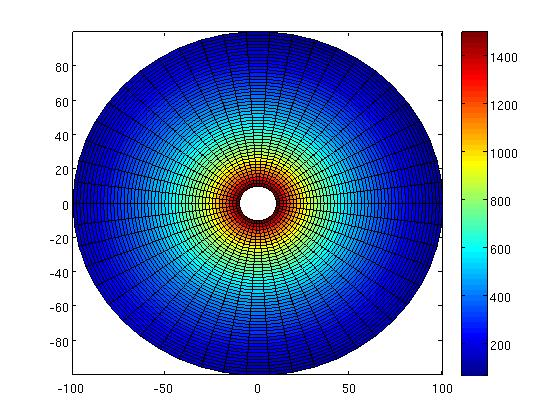
\includegraphics[width=10cm]{test5050atemp.jpg}
\label{Exp2Atemp}
\end{figure}

\begin{figure}[h!]
\centering
\caption{Grafico de temperaturas del experimento 2, caso B.}
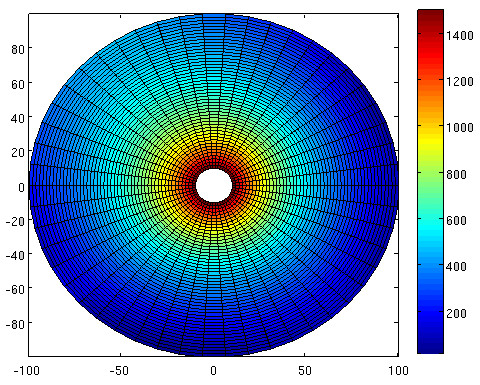
\includegraphics[width=8cm]{test5050btemp.jpg}
\label{Exp2Btemp}
\end{figure}

Luego, en base a estas temperaturas obtenidas, se utilizo el método de interpolación lineal para calcular la posición de la isoterma 500. En \ref{Exp1Aiso} \ref{Exp2Aiso} \ref{Exp3Aiso} y \ref{Exp4Aiso} se puede observar la ubicación de la isoterma, para cada una de los experimentos en el caso A. 

\begin{figure}[h!]
\centering
\caption{Grafico de la isoterma 500 del experimento 1, caso A.}
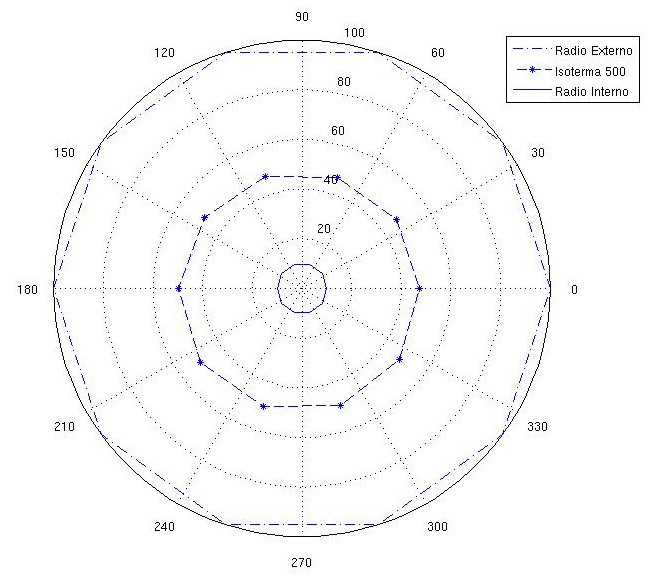
\includegraphics[width=8cm]{test1010aiso.jpg}
\label{Exp1Aiso}
\end{figure}

\begin{figure}[h!]
\centering
\caption{Grafico de la isoterma 500 del experimento 2, caso A.}
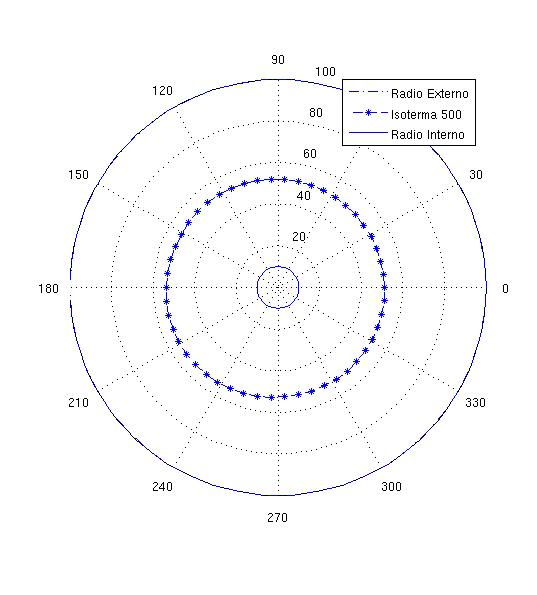
\includegraphics[width=7cm]{test5050aiso.jpg}
\label{Exp2Aiso}
\end{figure}

\begin{figure}[h!]
\centering
\caption{Grafico de la isoterma 500 del experimento 3, caso A.}
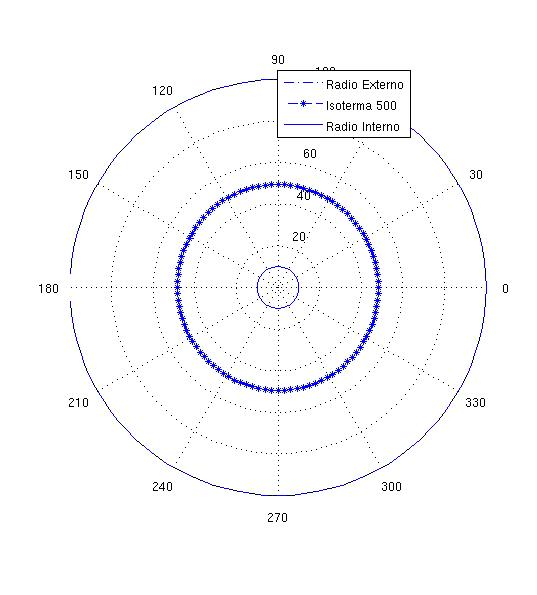
\includegraphics[width=7cm]{test20100aiso.jpg}
\label{Exp3Aiso}
\end{figure}

\begin{figure}[h!]
\centering
\caption{Grafico de la isoterma 500 del experimento 4, caso A.}
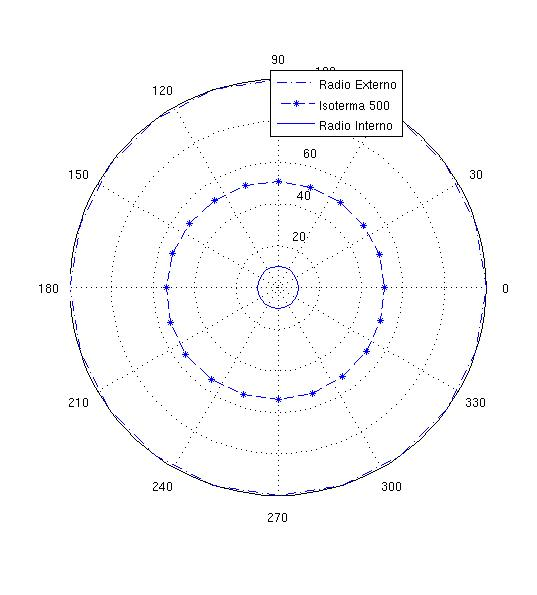
\includegraphics[width=7cm]{test10020aiso.jpg}
\label{Exp4Aiso}
\end{figure}

De la misma forma, para el caso B se llevaron a cabo los mismos experimentos como se puede observar en \ref{Exp1Biso} \ref{Exp2Biso} \ref{Exp3Biso} y \ref{Exp4Biso}

\begin{figure}[h!]
\centering
\caption{Grafico de la isoterma 500 del experimento 1, caso A.}
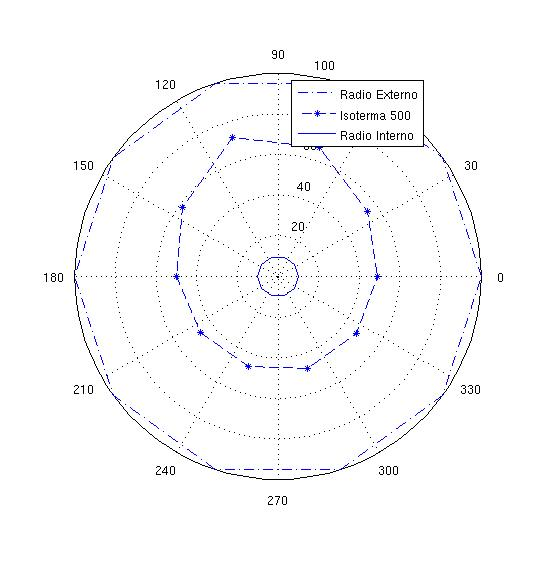
\includegraphics[width=7cm]{test1010biso.jpg}
\label{Exp1Biso}
\end{figure}

\begin{figure}[h!]
\centering
\caption{Grafico de la isoterma 500 del experimento 2, caso A.}
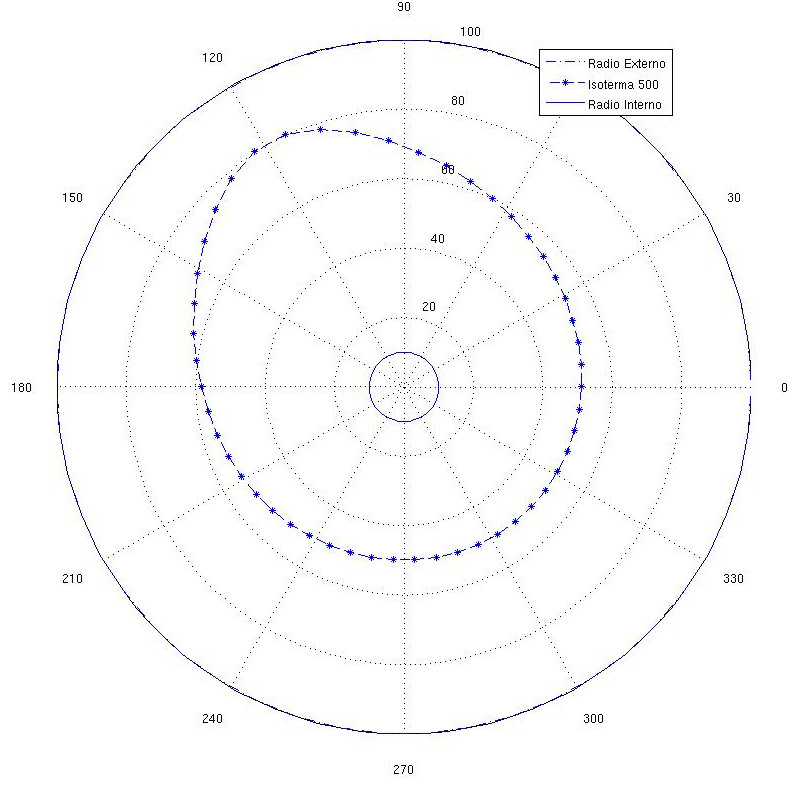
\includegraphics[width=7cm]{test5050biso.jpg}
\label{Exp2Biso}
\end{figure}

\begin{figure}[h!]
\centering
\caption{Grafico de la isoterma 500 del experimento 3, caso A.}
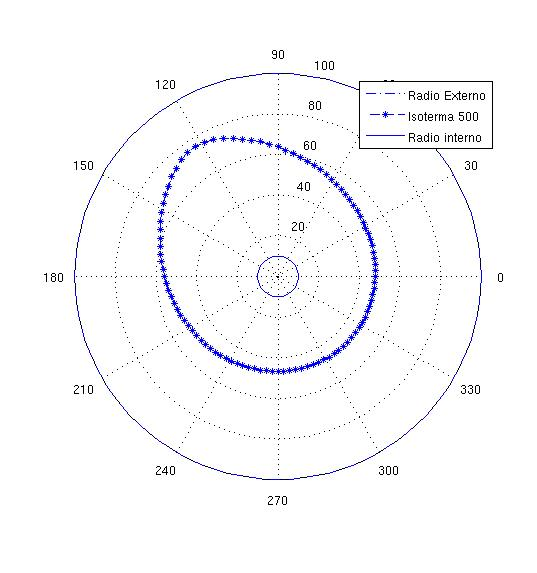
\includegraphics[width=7cm]{test20100biso.jpg}
\label{Exp3Biso}
\end{figure}

\begin{figure}[h!]
\centering
\caption{Grafico de la isoterma 500 del experimento 4, caso A.}
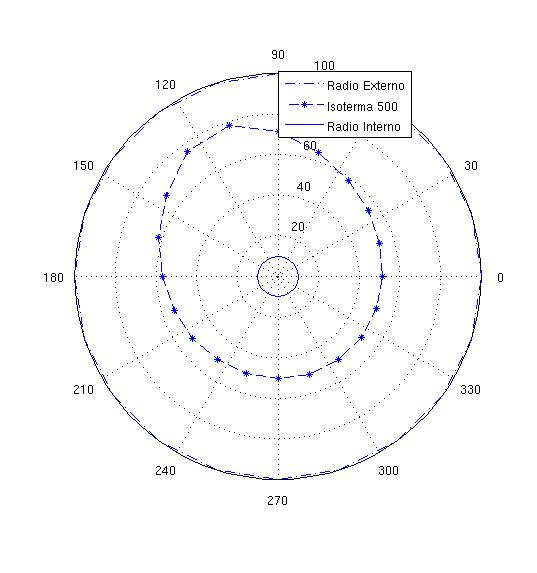
\includegraphics[width=7cm]{test10020biso.jpg}
\label{Exp4Biso}
\end{figure}

\subsubsection{Discusión de los resultados}

En un principio, antes de realizar los experimentos, pensabamos que llegaríamos a la conclusión de que una discretización pobre llevaría a resultados muy distintos a los obtenidos por una discretización más fina. Por ejemplo, esperabamos encontrarnos con algun caso de riesgo con temperaturas altas que el experimento 1 ignore, pero incluso éste resultó dar una aproximación bastante acertada. \\

Esto se puede deber a que por la forma en la que se trasmite el calor por la pared, dada por la ecuación de Laplace, no es posible que se registren altas temperaturas en un punto de la pared, sin que se vea reflejado de alguna forma en los puntos cercanos. \\
Esto se puede observar tambien comparando las \ref{Exp2Atemp} y \ref{Exp2Btemp}, donde claramente se ve el cambio gradual del calor, a pesar de la diferencia extrema de temperaturas registradas en la pared exterior. \\

\subsubsection{Experimentos 5 y 6}    

Con el objetivo de corroborar lo observado en los experimentos previos, se realizan dos nuevos experimentos. Además, se espera llegar a alguna conclución respecto a cual de los rangos de la discretización, la cantidad de ángulos o la cantidad de radios, es más importante para lograr un resultado fiable. \\

En \ref{Exp5Biso} se pueden observar los resultados superpuestos de variar la cantidad de ángulos $(N)$, dejando los radios fijos en 20. \\

De la misma forma, en  \ref{Exp6Biso} se ven los resultados de variar la cantidad de radios $(M+1)$, dejando fijos 20 ángulos.

\begin{figure}[h!]
\centering
\caption{Grafico de las isotermas 500 del experimento 5.}
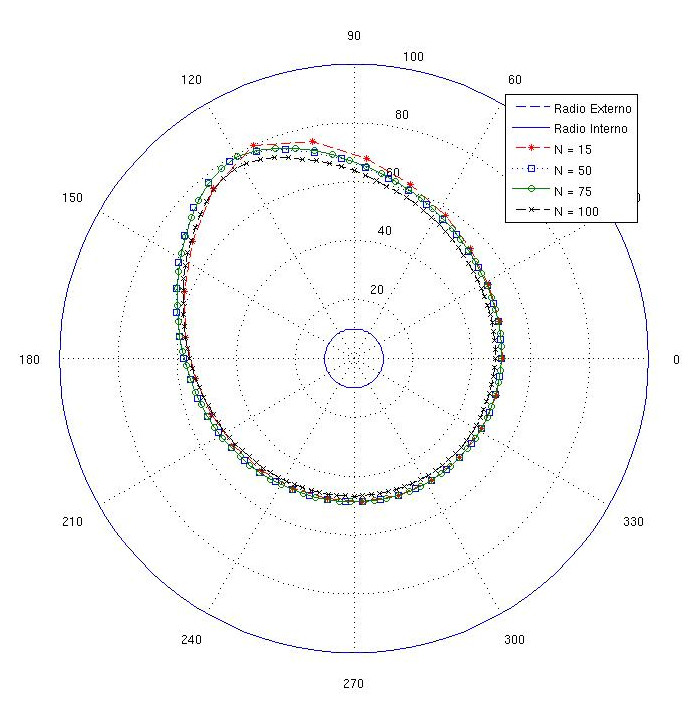
\includegraphics[width=8cm]{compare20N.jpg}
\label{Exp5Biso}
\end{figure}

\begin{figure}[h!]
\centering
\caption{Grafico de las isotermas 500 del experimento 6.}
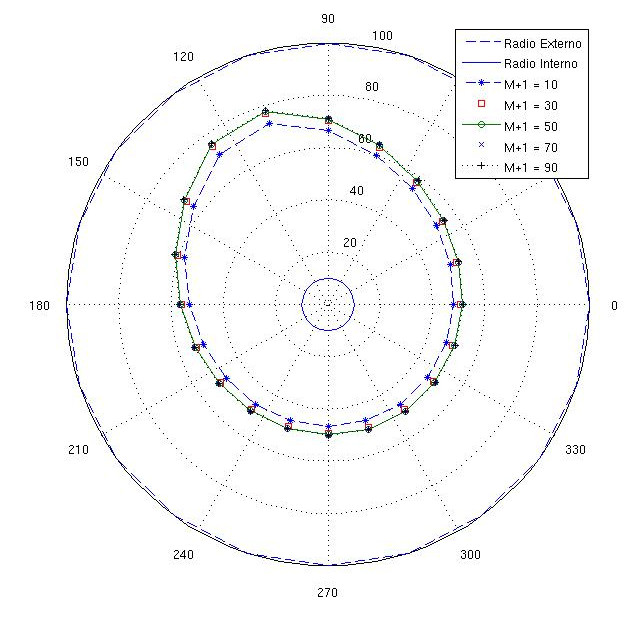
\includegraphics[width=9cm]{compareM20.jpg}
\label{Exp6Biso}
\end{figure}

\subsubsection{Discusión de los resultados}
Con estos nuevos experimentos, confirmamos lo observado en los experimentos 1 a 4. \\
En la \ref{Exp5Biso} vemos que el único experimento que devolvió un resultado alejado de los demás, es en el que usamos solamente 10 radios, pero que a partir de aumentar esta variable a 30 se equilibra el sistema y a partir de allí se consiguen resultados muy similares. \\
Siendo más exactos, la mayor diferencia entre el punto más cercano de la isoterma a la pared exterior obtenido con 30, 50, 70 y 90 radios se dió entre el resultado de M+1 = 30 y M+1 = 90, y es tan solo del orden de 1,2\% \\

\begin{equation}
\frac{ISO_{max}(M+1=90) - ISO_{max}(M+1=30)}{R_e - R_i} = \frac{77.935665
 - 76.818577}{100 - 10} = 0,012412089
\end{equation}

Sin embargo, y ésto es lo que más nos sorprendió, en la \ref{Exp5Biso} observamos que las diferencias entre las distintas aproximaciones de la isoterma es muy pequeña a pesar de la gran diferencia de los valores utilizados. Más aún, no parece haber una relación tan directa entre una discretización de ángulos más fina y un resultado más preciso. Por ejemplo, el resultado obtenido con 100 y con 15 ángulos tienen una diferencia de apenas 0,69\% entre si, pero de 5,7\% respecto del valor \"real" (obtenido con una discretización más fina y equilibrada de 100x100, que requirió varios minutos de cómputo)

\begin{equation}
\frac{ISO_{max}(N=100) - ISO_{max}(N=15)}{R_e - R_i} = \frac{75.872249 - 75.248781}{100 - 10} = 0,006927422
\end{equation}

En conclución, podemos inferir que no es efectivo tomar discretizaciones con valores de N y M muy diferentes, ya que aumentar una de las variables y no la otra, no necesariamente lleva a mejores resultados. Lo más eficiente es tomar una discretización equilibrada en N y M, sin necesidad de que sean valores muy altos, que requerirían mucho tiempo de cómputo. 

\subsection{Experimentos de Complejidad}

\subsubsection{Experimento 1}

En este experimento se esperaba ver como se comportaban temporalmente nuestras implentaciones de la Factorizacion LU y Eliminacion Gaussiana. Previamente se había demostrado de forma teórica que la complejidad de estos metodos era cúbica, por lo que se esperaba demostrar empíricamente que nuestra implementación cumplia con dicha complejidad.

\begin{figure}[h!]
\centering
\caption{Grafico del Tiempo de Resolucion del sistema usando E.G.}
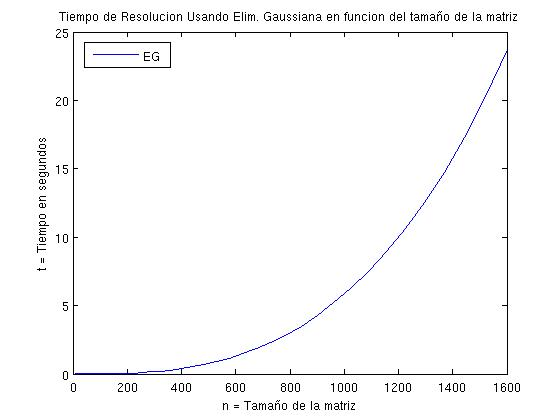
\includegraphics[width=10cm]{CTemporalEG.jpg}
\label{Exp1EG}
\end{figure}

\begin{figure}[h!]
\centering
\caption{Grafico del Tiempo de Resolucion del sistema usando Fact. LU}
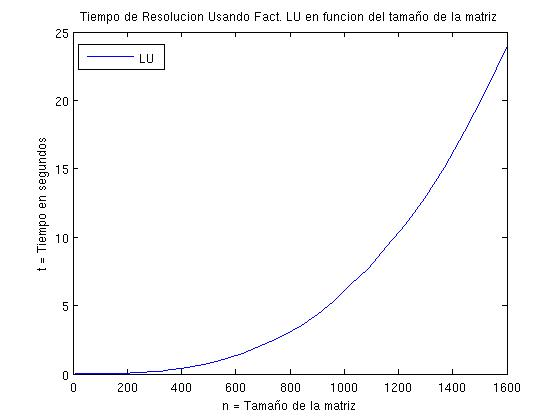
\includegraphics[width=10cm]{CTemporalLU.jpg}
\label{Exp1LU}
\end{figure}

Tanto en la \ref{Exp1EG}, como en la \ref{Exp1LU} se puede observar que la complejidad temporal crece en orden cubico como se habia previsto, esto se debe a que nuestros metodos son de cota inferior Cubica en peor caso, por lo que apesar de que nuestra implentacion no esta lo suficientemente optimizada para tener una constante minima, es bastante aceptable ya que como se ve en los graficos es de orden cubica.

\begin{figure}[h!]
\centering
\caption{Comparacion entre Fact.LU y E.G. del Tiempo de Resolucion del sistema}
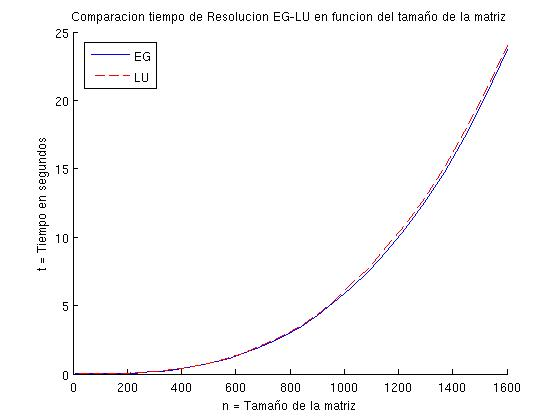
\includegraphics[width=12cm]{ComparacionLUEG.jpg}
\label{Exp1Comp}
\end{figure}

\subsubsection{Discusión de los resultados}

Una de las hipotesis que sosteniamos antes de las experimentacion es que Fact. LU iba a ser mejor que E.G., a pesar de ejecutar una sola instancia, esto como se puede observar en la \ref{Exp1Comp} es falso, aunque por un margen pequeño, suponemos que esto se debe a que mientras la E.G. solo triangula el sistema y resuelve un sistema triangular superior, Fact. LU tambien debe triangular el sistema y resolver un sistema triangular superior, y ademas debe resolver un sistema triangular inferior, por lo que el pequeño margen de tiempo debe encontrarse ahi.

\subsubsection{Experimento 2}
En este experimento se esperaba ver como variaba la complejidad temporal de nuestros metodos en funcion del numero de instancias a resolver. Esperabamos que Fact. LU fuera mejor que E.G., haciendo uso de las propiedades inertes al proceso de Fact. LU vistas en la teorica.
\\

\begin{figure}[h!]
\centering
\caption{Grafico del Tiempo de Resolucion del sistema usando E.G. para n instancias en una Matriz de 30x30}
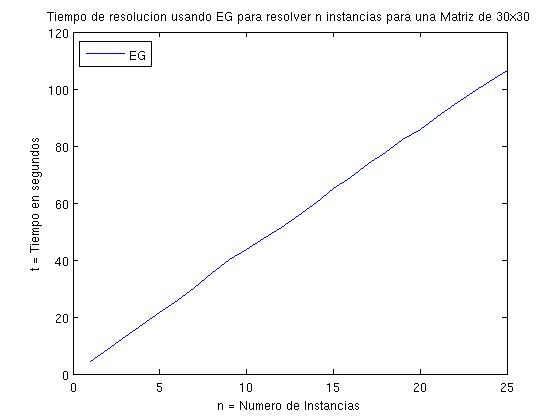
\includegraphics[width=10cm]{tmpPara25InstEG.jpg}
\label{Exp2EG}
\end{figure}

Como se puede ver en la \ref{Exp2EG}, el tiempo que tarda en resolver n instancias distintas usando E.G. es similar a:

$n$ x Tiempo para una instancia
Esto se debe principalmente a que debe triangular la matriz para cada instancia que ejecuta, por lo que para cada instanciar que resuelva debe volver a gastar tiempo cubico en triangularizar.

\begin{figure}[h!]
\centering
\caption{Grafico del Tiempo de Resolucion del sistema usando Fact. LU para n instancias en una Matriz de 30x30}
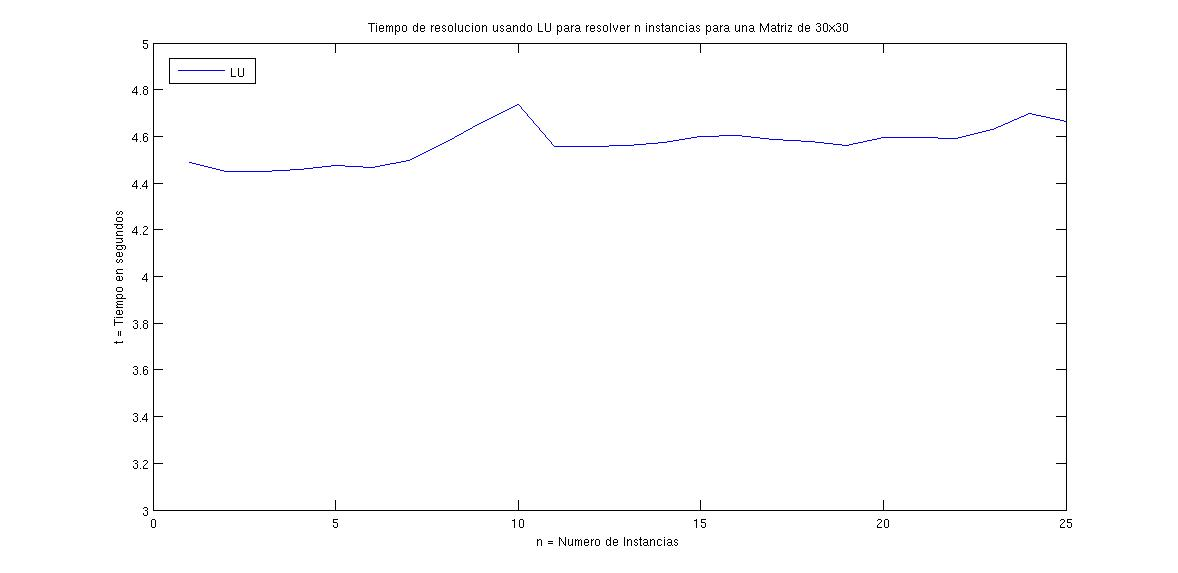
\includegraphics[width=16cm]{tmpPara25InstLU.jpg}
\label{Exp2LU}
\end{figure}
En la \ref{Exp2LU}, en cambio observamos que usando Fact. LU resolver una instancia o numero mucho mayor de estas no repercute perceptiblemente en la complejidad temporal, en este caso al tener la Fact. LU la propiedad que para resolver un sistema:
A$\cdot$ x $=$ b, se puede resolver los sistemas A $=$ L $\cdot$ U, L $\cdot$ y $=$ b y U$\cdot$ x $=$ y.
Por lo que de esta forma solo es necesario triangular la matriz en la primera instancia, y en las siguientes solo se debe resolver dos matrices triangular inferior y superior respectivamente, lo que hace que en las siguientes instancias el tiempo sea minimo. 
\begin{figure}[h!]
\centering
\caption{Comparacion entre Fact.LU y E.G. del Tiempo de Resolucion del sistema para n instancias en una Matriz de 30x30}
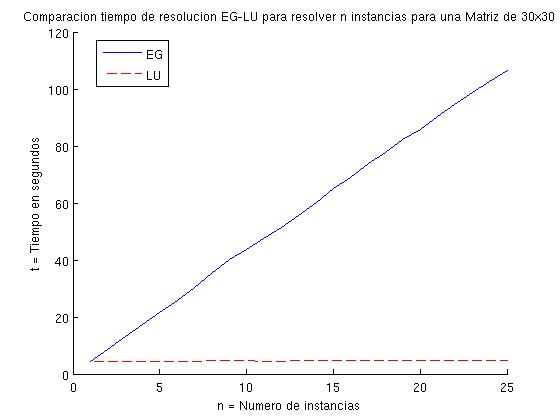
\includegraphics[width=12cm]{CompLUEGpara25Inst.jpg}
\label{Exp2Comp}
\end{figure}

En la \ref{Exp2Comp} se puede ver claramente que mientras la Fact. LU es practicamente constante con respecto al numero de instancias a resolver, la E.G. es lineal. Este resultado fue una de las cosas que motivaron la realizacion del experimento tres con el fin de terminar de comprobar las hipotesis planteadas en las conclusiones de este experimento.

\subsubsection{Experimentos Tres}

En este experimento fue motivado apartir de los resultados obtenidos en el experimento dos,se esperaba comprobar dos cosas que la complejidad para resolver la instancia numero uno o la iesima era constante, o practicamente la misma en la E.G. y que en el caso de la Factorizacion LU la instancia numero uno era la que cargaba como el factor temporal dominante y el tiempo de resolucion de las siguientes era casi despreciable. Para esto se ideo un test donde se media el tiempo que tomaba resolver la instancia uno a la diez para una matriz de 30x30.
\begin{figure}[h!]
\centering
\caption{Grafico del Tiempo de Resolucion de cada instancia particular usando E.G. para 10 instancias en una Matriz de 30x30}
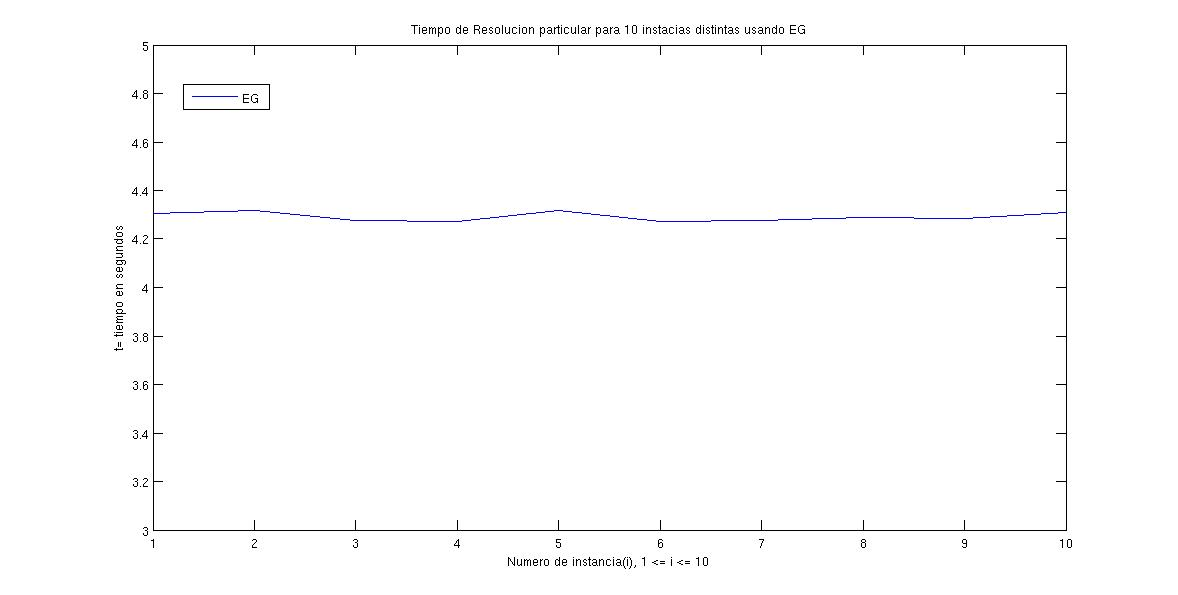
\includegraphics[width=16cm]{tmp10InstFijasEG.jpg}
\label{Exp3EG}
\end{figure}

En la \ref{Exp3EG} se ve claramente como el tiempo que toma resolver cualquier instancia es practicamente el mismo, esto se produce a que para cada instancia debe resolver el sistema entero, por ser un algoritmo poco eficiente en terminos de reusabilidad.
\begin{figure}[h!]
\centering
\caption{Grafico del Tiempo de Resolucion de cada instancia particular usando Fact. LU para 10 instancias en una Matriz de 30x30}
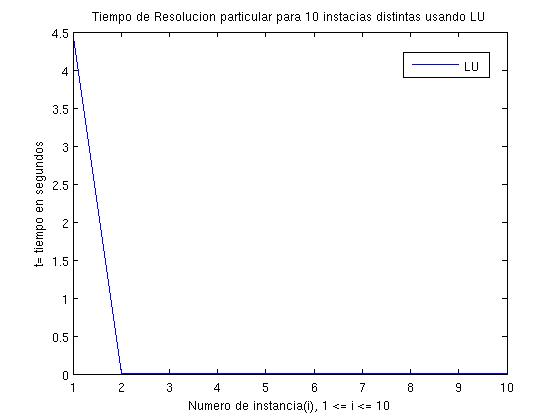
\includegraphics[width=12cm]{tmp10InstFijasLU.jpg}
\label{Exp3LU}
\end{figure}
\\
En la \ref{Exp3LU} se ve como se comfirma la hipotesis inicial de que la complejidad temporal es consumida mayormente en factorizar la matriz y que la resolucion de los sistemas ya triangulados es despreciable temporalmente hablando.
\begin{figure}[h!]
\centering
\caption{Comparacion entre Fact.LU y E.G. del Tiempo de Resolucion de cada instancia particular para 10 instancias en una Matriz de 30x30}
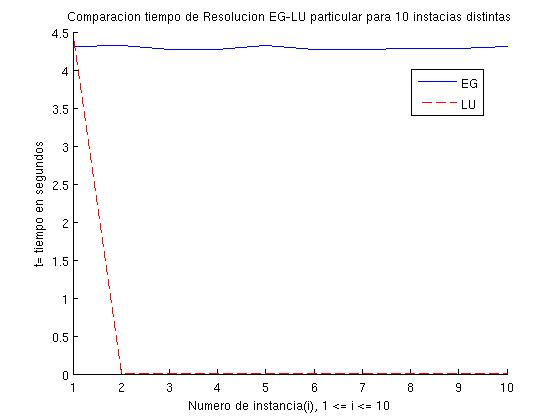
\includegraphics[width=13cm]{CompLUEG10InstFijas.jpg}
\label{Exp3Comp}
\end{figure}
\\
Para representar mas visualmente  la diferencia entre Factorizacion LU y Eliminacion Gaussiana se presenta en la \ref{Exp3Comp} una comparacion donde se observa claramente la diferencia de rendimiento entre Factorizacion LU y E.G. luego de ejecutar la primera instancia, esto como se infirio anteriormente tiene que ver con la obligatoriedad en el caso de E.G. de tener que triangular en cada instancia la matriz del sistema. 

\subsubsection{Experimento Cuatro}

El objetivo de este experimento es analizar la exactitud de los métodos implementados.\\
Elegimos crear dos instancias de un sistema pequeño, con $N = 5$ y $M+1 = 5$, ya que esto generará dos vectores resultado de tamaño 25, de los cuales 10 son triviales, y consideramos los 15 resultados suficientes para evaluar en promedio cual es el error generado. \\

Entendemos que Matlab debe utilizar los algoritmos con las mejores optimizaciones posibles por lo que tomamos estos resultados como representativos de los resultados reales. 

El primer paso del experimento consistió en resolver las dos instancias del sistema con los dos metodos implementados, pero nos encontramos con que, tal como esperabamos, conseguimos exactamente los mismos resultados. Por lo tanto, para el resto del experimento no hará falta comparar cada uno de los resultados por separado. Nos referiremos a los resultados obtenidos con cualquiera de los dos metodos como $v1$ y $v2$

Los resultados obtenidos con Matlab, a los que llamaremos $m1$ y $m2$, se compararon como se puede ver en la \ref{CompML} en la que, para cada instancia, no se puede notar a simple vista ninguna diferencia ya que los gráficos se superponen.

\begin{figure}[h!]
\centering
\caption{Comparación de los resultados contra Matlab}
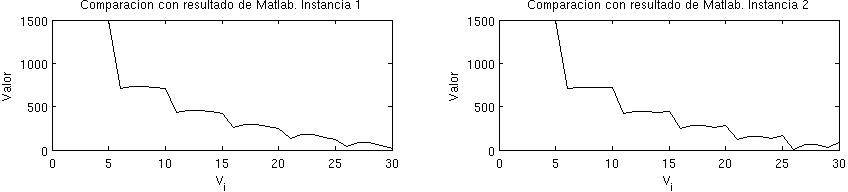
\includegraphics[width=17cm]{ComparacionML.jpg}
\label{CompML}
\end{figure}

Para poder sacar conclusiones respecto del experimento, procedimos a restar $m1 - v1$ y a esto dividirlo componente a componente por m1. De la misma forma con la segunda instancia $v1$ y $m1$ para obtener dos vectores a los que llamamos Diferencia Relativa, o $d1$ y $d2$.\\

En la \ref{VectorResta} se pueden ver los valores de estas diferencias, o observamos que estan en el orden de las milésimas.  

\begin{figure}[h!]
\centering
\caption{Valores del vector D}
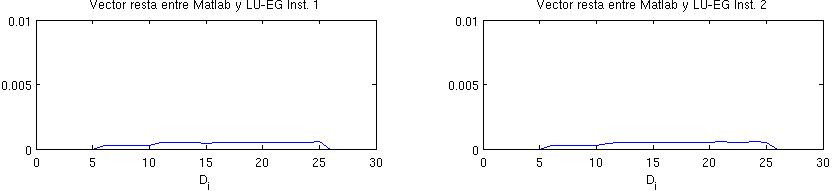
\includegraphics[width=17cm]{VectorRestaRelativa.jpg}
\label{VectorResta}
\end{figure}

\subsubsection{Discusión de los resultados}

Las conclusiones obtenidas en estos experimentos son que si bien en complejidad teorica los dos metodos empleados se comportan de la misma manera, es decir tienen complejidad cubica en la practica, a la hora de resolver sistemas donde se puedan presentar muchas instancias distintas a resolver en el futuro es altamente recomendable usar Factorizacion LU, por sobre E.G., ya que usar E.G. y no Fact. LU para resolucion de un gran numero de instancias, puede ser enormemente perjudicial en terminos de rendimiento. \\

Por otra parte, quedó demostrado que aunque nuestros algoritmos parecian perfectos, la sucesión de operariones sobre numeros densos en los reales representados de manera discreta generó un error no despreciable. 
Sin embargo consideramos que en el contexto utilizado, el error obtenido es, aunque no despreciable, al menos aceptable.


\section{Conclusiones}

Algunas de las conclusiones obtenidas luego de la elaboracion de este informe y de haber llevado a cabo diferentes experimentos:
\begin{itemize}
\item Con respecto a la relación que hay entre el tamaño de la discretización del sistema y la precisión de los resultados con respecto a la isotermia buscada, concluimos que a partir de una cierta granulación de tamaño medio y equilibrado en sus variables, por ejemplo tomando 30 ángulos y 30 radios, no se encontraron diferencias significativas en la ubicación de la isotermia, con respecto a granulaciones de órden superior, como se puede ver en los experimentos. \\

Además, notamos que crear discretizaciones dispares, como tomar una amplia cantidad de ángulos y pocos radios o viceversa, no llevaba a resultados satisfactorios en comparación a una distribución equilibrada de ángulos y radios, con matriz resultante de similar tamaño, y por lo tanto tiempo de computo equivalente.

\item Con respecto a la complejidad de los métodos utilizados para resolver el sistema, se llegó a la conclución que, como era esperado, éstos se comportan con una complejidad de órden cúbico. Sin embargo, tambien se pudo observar que al trabajar con un gran numero de instancias, la factorización LU es ampliamente superior en terminos de complejidad temporal con respecto a la eliminación Gaussiana. 
Por otro lado, como ya describimos en la discución de resultados de los experimentos, se puede ver que la implementación de nuestros métodos no esta libre de error. Conciderando que trabajamos con aritmética finita y algoritmos poco optimizados nos encontramos con errores aceptables.
Además, se puede concluir que el gran problema de la resolucion de sistemas lineales no pasa por la resolucion del sistema en si, sino por convertir el sistema en uno amigable. Por lo que las lineas de investigacion deberian centrarse en ello.

\item Algunas de las posibles optimizaciones podrían ser las de aplicar pivoteo parcial al algoritmo de EG, y utilizar Factorización PLU para reducir estos errores de compúto ya que como se probó en las clases teóricas, usar pivoteo total y/o parcial al posicionar numeros grandes sobre la diagonal de nuestra matriz, se reduce la posibilidad de dividir por numeros pequeños lo cual minimiza el error.
Por otra parte, otra optimización realizable y que inferiría seguramente de forma positiva con respecto a la exactitud en la búsqueda de la isoterma, sería usar métodos de interpolación más eficientes, como por ejemplo el método de interpolación de Lagrange.

\end{itemize}

%Esta seccion debe contener las conclusiones generales del trabajo. Se deben mencionar
%las relaciones de la discusion sobre las que se tiene certeza, junto con comentarios
%y observaciones generales aplicables a todo el proceso. Mencionar tambien posibles
%extensiones a los metodos, experimentos que hayan quedado pendientes, etc.

\section{Apendices}

\subsection{Enunciado}

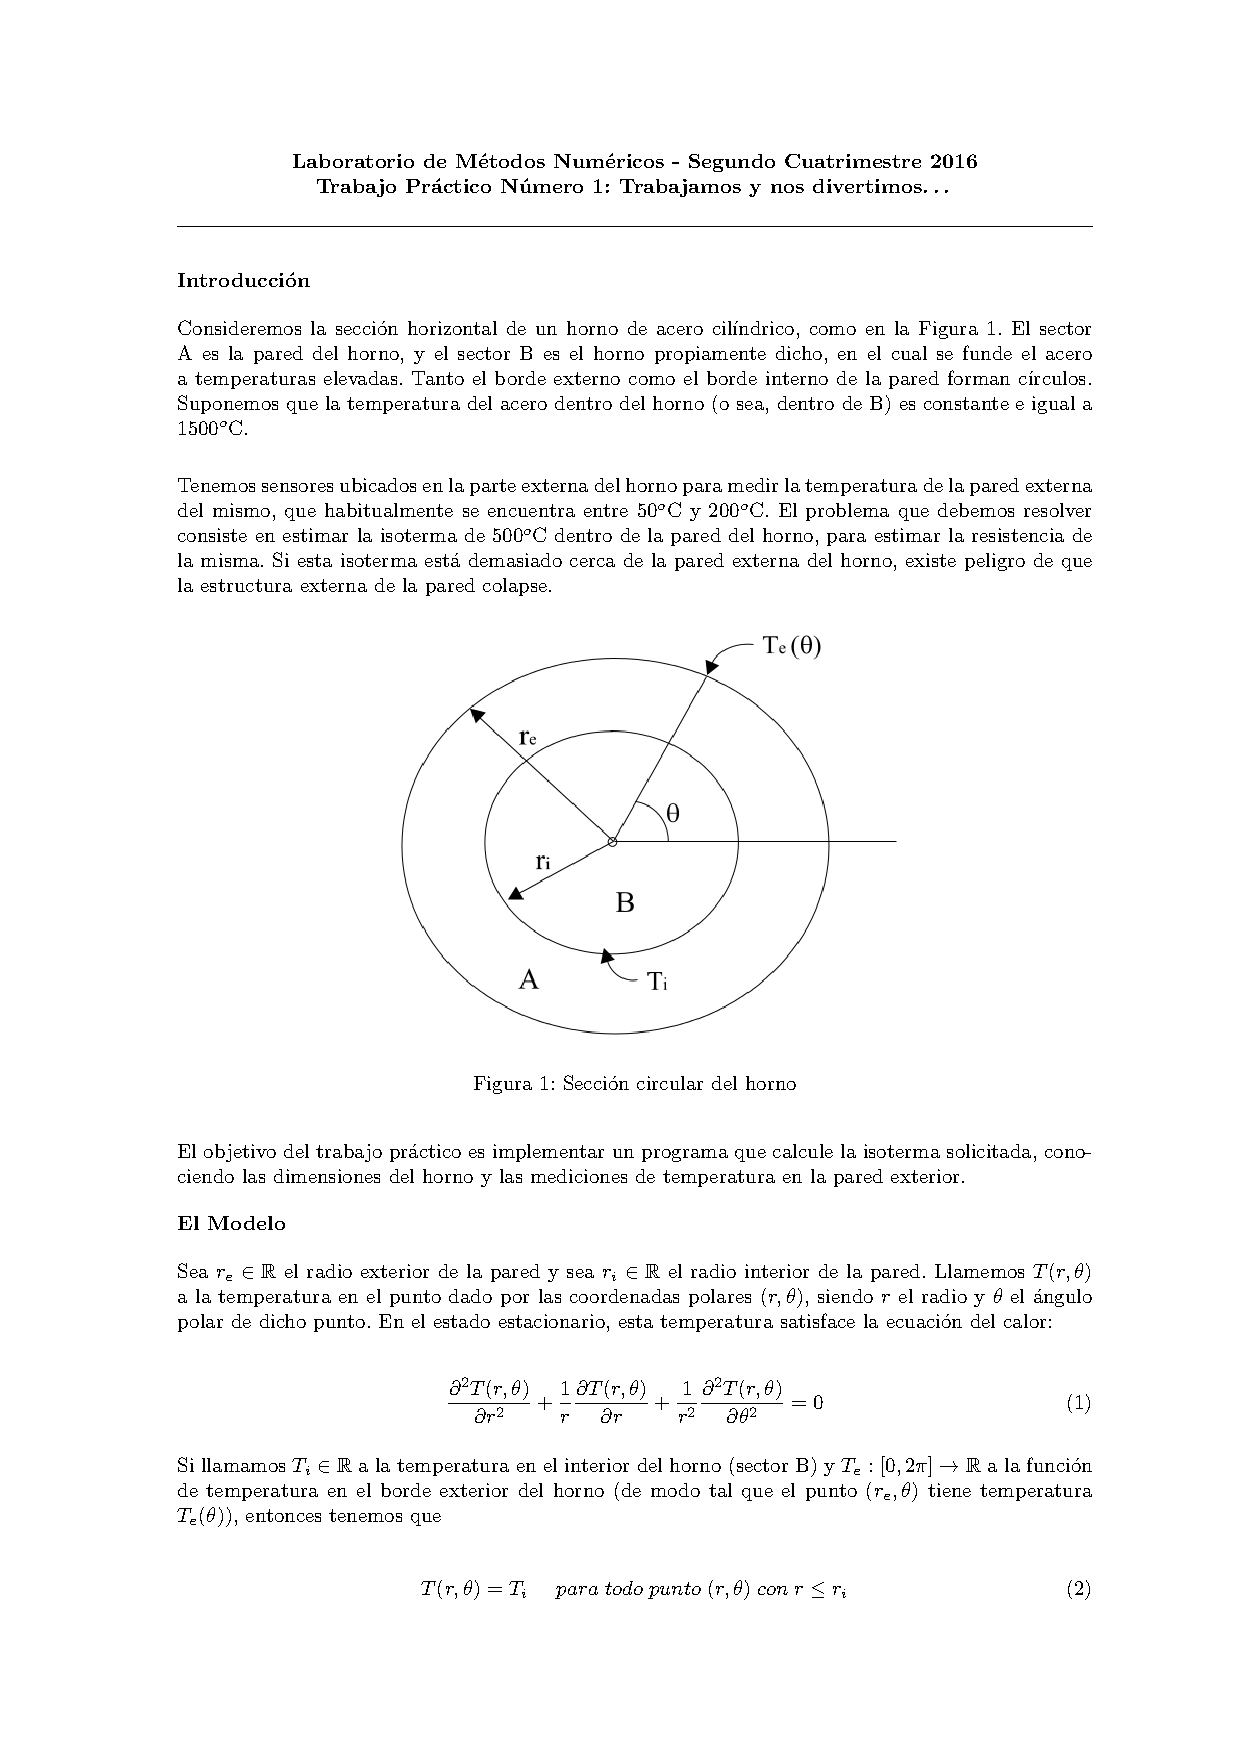
\includepdf[pages=-]{tp1.pdf}

\subsection{Codigo fuente}
A continuación se incluyen los los codigos fuente de las funciones relevantes desde el punto de vista numerico.

\subsubsection{Eliminación Gaussiana}
\begin{lstlisting}
void Matriz::EG(){
  int c = columnas();
  int f = filas();
  for (int i = 0; i < f-1; i++){
    for(int j = i+1 ; j < f; j++){
      double multiplicador = _matriz[j][i]/(double)_matriz[i][i];
      for (int k = i ; k < c ; k++){
        _matriz[j][k]=_matriz[j][k]-multiplicador*(double)_matriz[i][k];
      }
    }
  }
}
\end{lstlisting}

\subsubsection{Factorización LU}
(guardando L y U en la misma matriz)
\begin{lstlisting}
void Matriz::LU(){
  int c = columnas();
  int f = filas();
  for (int i = 0; i < f-1; i++){
    for(int j = i+1 ; j < f; j++){
      double multiplicador = _matriz[j][i]/(double) _matriz[i][i];
      for (int k = i ; k < c ; k++){
        if(k != i){
            _matriz[j][k] = _matriz[j][k] - multiplicador*(double) _matriz[i][k];
        }
        else{
            _matriz[j][k] = multiplicador;
        }
      }
    }
  }
}
\end{lstlisting}

\subsubsection{Backward Substitution}
\begin{lstlisting}
vector<double> Matriz::resolverTS(vector<double> b){
	vector<double> res(_filas, 0);
	for(int i = _filas-1; i>=0; i--){
		double acc = 0;
		for(int j = i+1; j<= _columnas-1; j++){
			acc += _matriz[i][j] *(double) res[j];
        }
		res[i] = (b[i]-acc)/(double) _matriz[i][i];
	}
	
	return res;
}
\end{lstlisting}

\subsubsection{Forward Substitution}
\begin{lstlisting}
vector<double> Matriz::resolverTI(vector<double> b){
	vector<double> res(_filas, 0);
	for(int i = 0; i< _filas; i++){
		double acc = 0;
		for(int j = 0; j < i ; j++){
			acc += _matriz[i][j] *(double) res[j];
        }
		res[i] = (b[i]-acc)/(double) _matriz[i][i];
	}
	
	return res;
}
\end{lstlisting}

\subsection{Proposición 1}
Sea $A \in \mathds{R}^{nxn}$ la matriz generada para el sistema del alto horno, es posible aplicar Eliminación Gaussiana sin pivoteo.

\subsubsection{Demostración}
Inicialmente se sabe que nuestra matriz es diagonal dominante y banda. Por la composición de nuestra matriz sabemos que esta no sólo no es nula sino que ninguna fila lo es.

Además por el armado de la matriz se sabe que el coeficiente de $t_{j,k}$ es:

\begin{align*}
t_{j,k}(- \frac{2}{(\Delta r)^2} + \frac{1}{r \Delta r} - \frac{2}{r^2 (\Delta \theta)^2})
\end{align*}

llamemos lo que multiplica a  $t_{j,k}$, $I_{j,k}$, se puede ver que $I_{j,k} \neq 0$ entonces sabemos que los elementos de la diagonal son no nulos ($a_{i,i} \neq 0 \forall i$).

Además sobre $t_{j-1,k}$ y $t_{j+1,k}$ se puede inferir lo siguente:
\begin{itemize}
\item $t_{j-1,k}(\frac{1}{(\Delta r)^2} - \frac{1}{r\Delta r})$, llamemos lo que multiplica a  $t_{j-1,k}$, $I_{j-1,k}$. $I_{j-1,k} \neq 0$, ya que si $I_{j-1,k} = 0$ entonces $(\Delta r)^2 = r \Delta r \Rightarrow r = \Delta r$ y esto solo pasa si no granulamos el radio.

\item $t_{j+1,k}(\frac{1}{(\Delta r)^2})$ llamemos lo que multiplica a  $t_{j+1,k}$, $I_{j+1,k}$. Se tiene trivialmente que $I_{j-1,k} > 0$
\end{itemize}

Además se sabe que el armado de las filas de la matriz es de la forma:

$
A = 
 \begin{pmatrix}
  I & \ldots & \ldots & \ldots & 0 \\
  \ddots & I_{j,k} & \ldots & I_{j+1,k} & 0 \\
  0 & \ddots & \ddots & \ddots & \cdots \\
  0 & 0 & \ddots & \ddots & I
 \end{pmatrix}
$

Veamos que luego de aplicar el primer paso de E.G. La matriz $\widetilde{A} \in {\mathds{R}}^{(n-1)x(n-1)}$ sigue siendo diagonal dominante con diagonal $\widetilde{a_{i,i}} \neq 0 ,\forall i$ y banda superior distinta de 0.

Es trivial que puedo aplicar sobre las primeras n filas identidad y tambien sobre el primer $I_{j,k}$ encontrado también ya que $I_{j,k} \neq 0$. También es trivial ver que los $I_{j+1,k}$ no cambian ya que arriba de ellos solo hay ceros, por lo que los $\widetilde{I_{j+1,k}}$ de $\widetilde{A}$ siguen siendo distintos de 0, ya que $\widetilde{I_{j+1,k}}$ $=$ ${I_{j+1,k}}$ .

Veamos que $\widetilde{A}$ sigue siendo diagonal dominante con $\widetilde{a_{i,i}} \neq 0$. Por la estructura del algoritmo de EG se realiza el siguiente paso:

\begin{align}
F_i - \frac{a_{i,1}}{a_{1,1}} F_1 \quad \forall i = 2 ... n \Rightarrow \widetilde{a_{i,j}} = a_{i,j} - \frac{a_{i,1}}{a_{1,1}} a_{i,j}
\end{align}

Sea

\begin{align*}
\sum ^{n}_{j \neq i} \left| \widetilde{a_{i,j}} \right| = \sum ^{n}_{j \neq i} \left| a_{i,j} - \frac{a_{i,1}}{a_{i,i}} a_{1,j} \right| \leq \sum ^{n}_{j\neq i; 2\leq j} \left| a_{i,j} \right| + \sum ^{n}_{j\neq i; 2\leq j} \left| \frac{a_{i,1}}{a_{1,1}} a_{1,j} \right|
\end{align*}

Como $\sum^n_{j\neq i; 2\leq j} \left| a_{i,j} \right| \leq \left| a_{i,i} \right| $, por hipótesis de diagonal dominante:

\begin{align*}
\sum ^{n}_{j\neq i; 2\leq j} \left| a_{i,j} \right| + \sum ^{n}_{j\neq i; 2\leq j} \left| \frac{a_{i,1}}{a_{1,1}} a_{1,j} \right| \leq \left| a_{i,i} \right| - \left| a_{i,1} \right| + \left| \frac{a_{i,1}}{a_{1,1}} \right| \sum ^n_{j\neq i; 2\leq j} \left| a_{1,j} \right|
\end{align*}

Como $\sum^n_{j\neq i; 1\leq j} \left| a_{1,j} \right| \leq \left| a_{1,1} \right|$ por hipótesis de diagonal dominante:

\begin{align*}
 \left| a_{i,i} \right| - \left| a_{i,1} \right| + \left| \frac{a_{i,1}}{a_{1,1}} \right| \sum ^n_{j\neq i; 2\leq j} \left| a_{1,j} \right| \leq \left| a_{i,i} \right| - \left| a_{i,1} \right| + \left| \frac{a_{i,1}}{a_{1,1}} \right| \left( \left| a_{1,1} \right| - \left| a_{1,i} \right| \right) = \left| a_{i,i} \right| - \left| \frac{a_{i,1}}{a_{1,1}} \right| \left|a_{1,i} \right|
\end{align*}

Que por (7)

\begin{align*}
\sum ^n_{j\neq i} \left| \widetilde{a_{i,j}} \right| \leq \left| a_{i,i} \right| - \left|\frac{a_{i,1}}{a_{1,1}} a_{1,i} \right| = \left| \widetilde{a_{i,i}} \right| \forall i
\end{align*}

Además como $I_{j+1,k}$ no es modificado por lo visto anteriormente y $I_{j+1,k}$ esta dentro del conjunto de los $\{ \widetilde{a_{i,j}} \}_{j\neq i; i fijo}$, por lo que se tiene que:

\begin{align*}
0 < \left| I_{j+1,k} \right| \leq \sum _{j \neq i} \left| \widetilde{a_{i,j}} \right| \leq \left| \widetilde{a_{i,i}} \right| \Rightarrow \left| \widetilde{a_{i,i}} \right| > 0
\end{align*}

Entónces $\widetilde{A}$ es diagonal dominante, con $\widetilde{a_{i,i}} \neq 0$ y no altera la banda superior. Usando un razonamiento inductivo sobre $\widetilde{A}$, se puede ver fácilmente que se le puede aplicar E.G sin pivoteo ya que al aplicar el primer paso de E.G sobre A obtengo un sistema $\widetilde{A} \in \mathds{R}^{(n-1)x(n-1)}$ de con las misma propiedades relevantes para esta demostracion. $\square$
\section{Referencias}

http://www.cplusplus.com/

http://stackoverflow.com/

https://en.wikipedia.org/wiki/Blast\_furnace 

http://linux.die.net/man/1/time

http://stackoverflow.com/questions/556405/what-do-real-user-and-sys-mean-in-the-output-of-time1

Ademas en temas referidos al armado del sistema y errores de presicion en la implementacion, asi como en la propiedad a demostrar dialogamos con otro grupo que se habia topado con barreras similares a las nuestras. 
\end{document}
